\section{溶液作製精度に関して}

溶液の作製精度の確認を行うため,0.95,1.00,1.05wt.\%のPAA溶液を作成した.それぞれの溶液の特性を確認するため,粘度計を用いて粘度計測を行った.粘度計測を行った結果をFig.\ref{fig:95-105}に示す.濃度が薄いと粘度は低く,濃度が高いと粘度は高くなった.

ぞれぞれの質量濃度のPAA溶液に対し,落下球実験を行った.落下させた球は,鋼製の直径10mmの球である.

\begin{figure}[ht]
    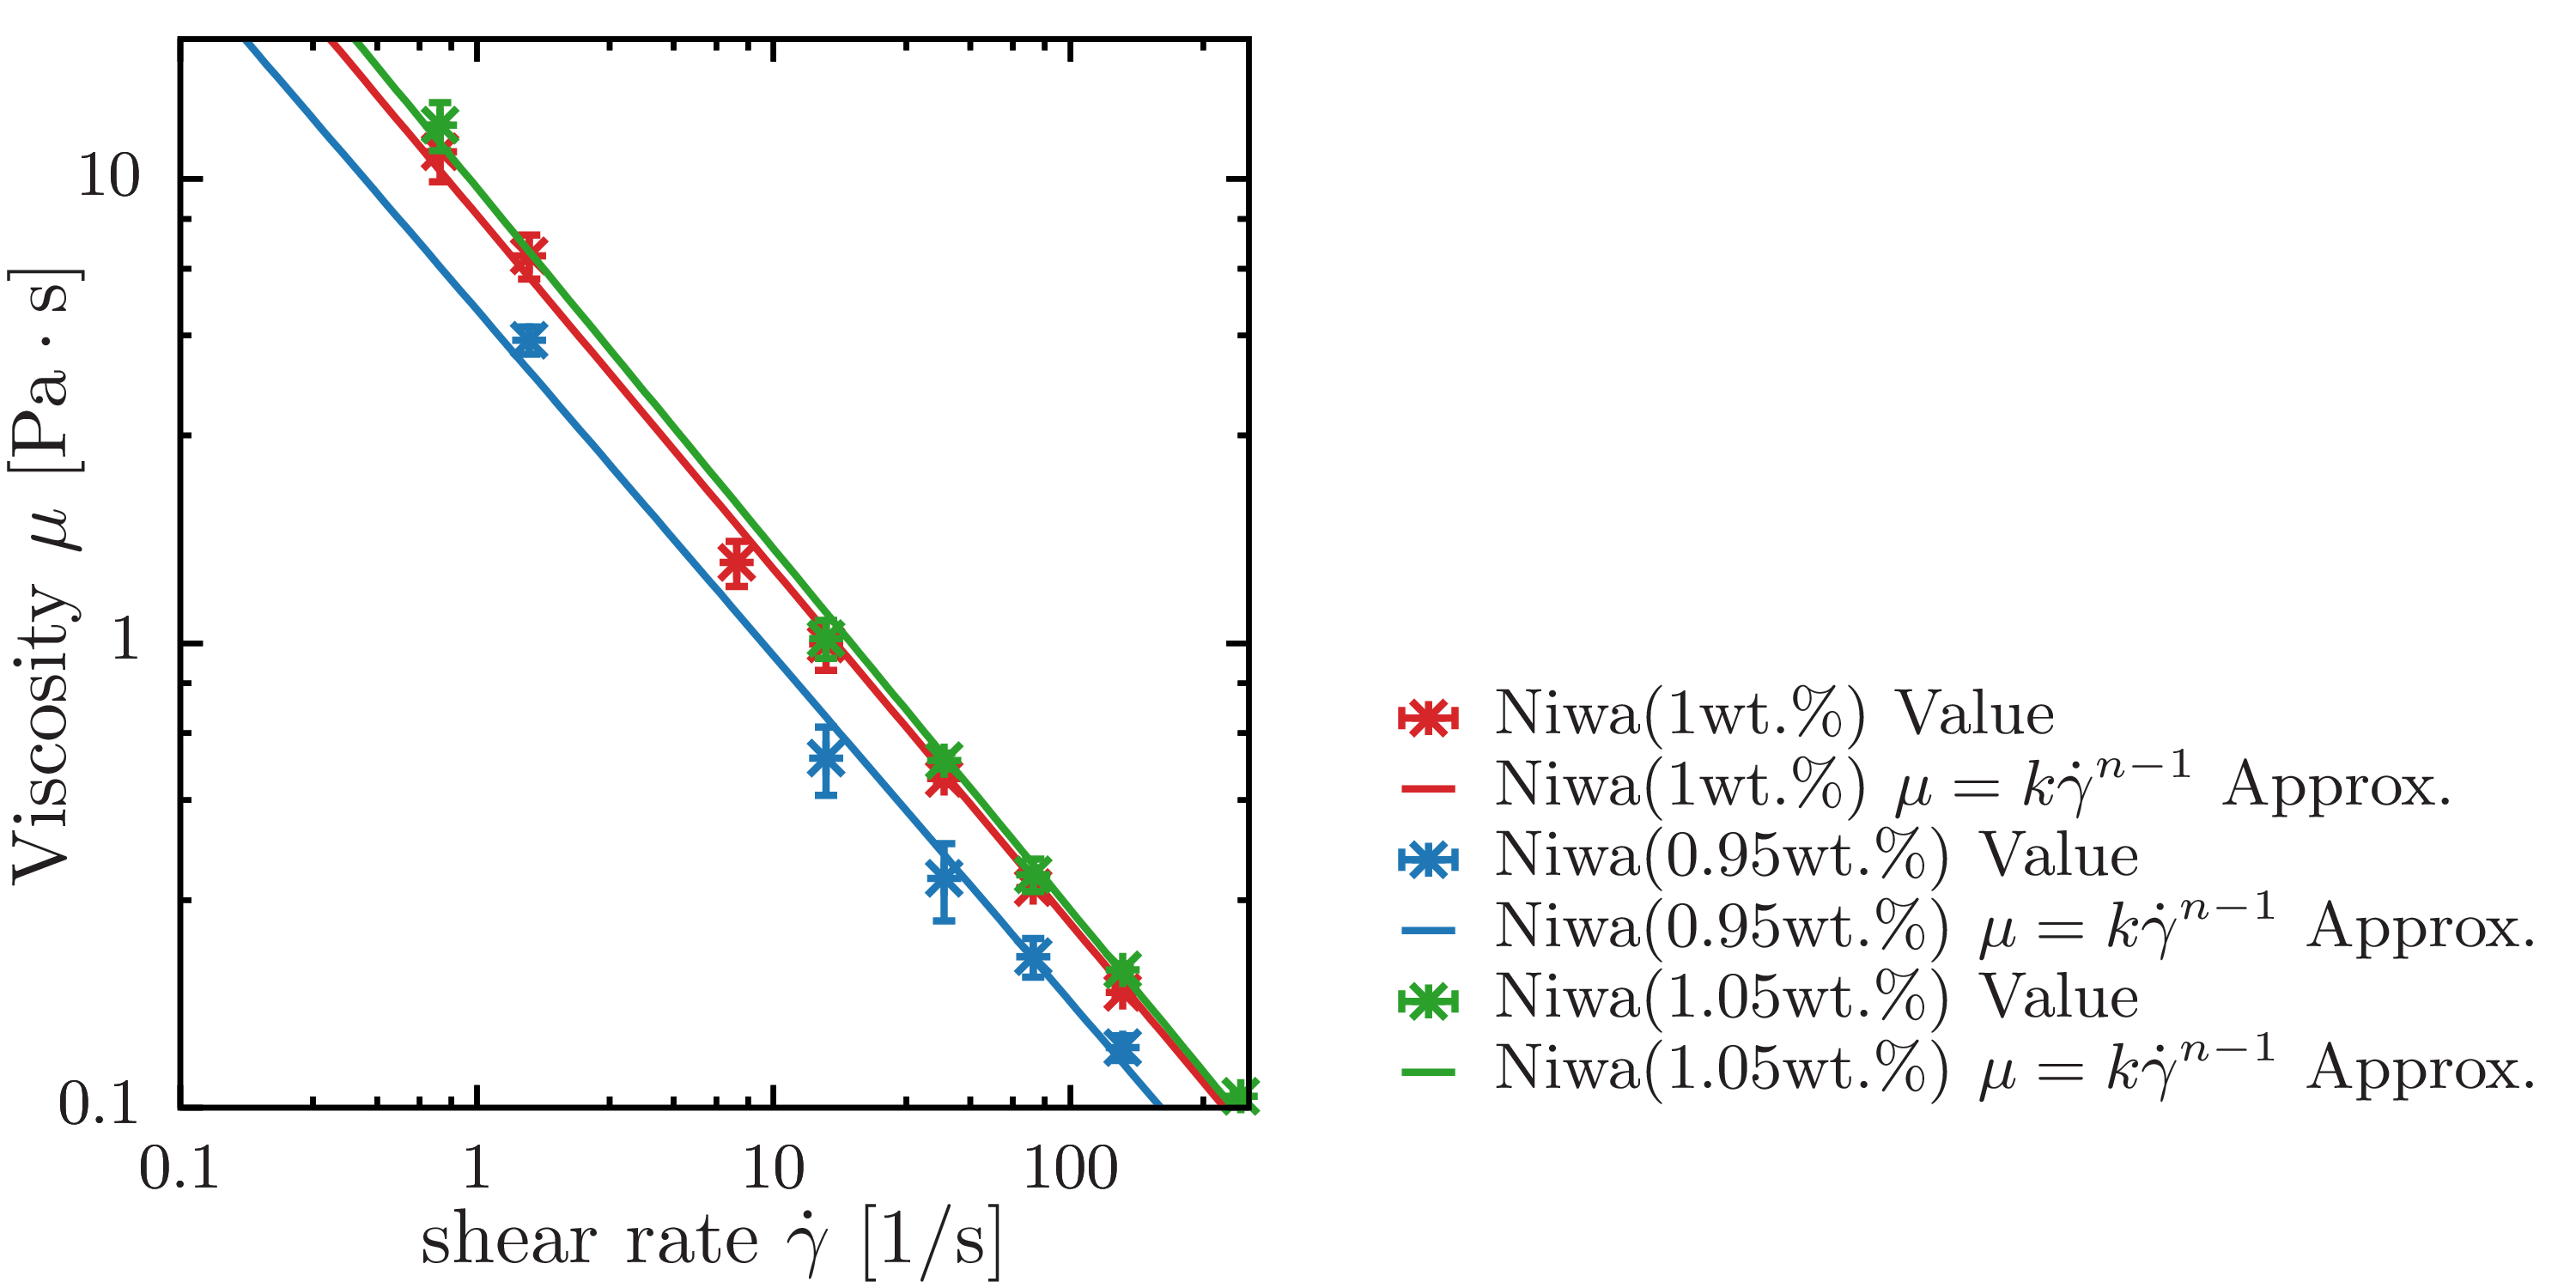
\includegraphics[width=15cm,clip]{5-Discussion/95-105.png}
    \caption{Flow curve for 0.95~1.05wt.\%PAA solution.}
    \label{fig:95-105}
\end{figure}

